% !TeX root = ../thuthesis-example.tex

\chapter{基于轻量级上下文切换的后训练通信优化}

\section{概述}
大语言模型对齐近来备受关注。
% ,凸显了确保这些先进人工智能系统以符合伦理规范且有益社会的方式运行的必要性。
InstructGPT\cite{ouyang2022instructgpt}、ChatGPT\cite{chatgpt} 系列模型(包括 OpenAI 的 GPT-4 \cite{openai2023gpt4}、谷歌的 Bard\cite{bard}以及 Meta 的 LLama-2-Chat \cite{touvron2023llama})的最新发展,都强调了对齐在这些模型中的重要性。
实现这种对齐的主要方法是基于人类反馈的强化学习(RLHF),其中近端策略优化(PPO)是广泛认可的标准算法,它显著提升了大语言模型在包括自然语言处理\cite{chatgpt,kreutzer2018reliability}、文本生成图像\cite{wu2023visualchatgpt,lee2023aligning}等诸多深度学习任务中的可靠性。 

\begin{figure}[ht]
    \centering
    % \resizebox{\linewidth}{!}{
    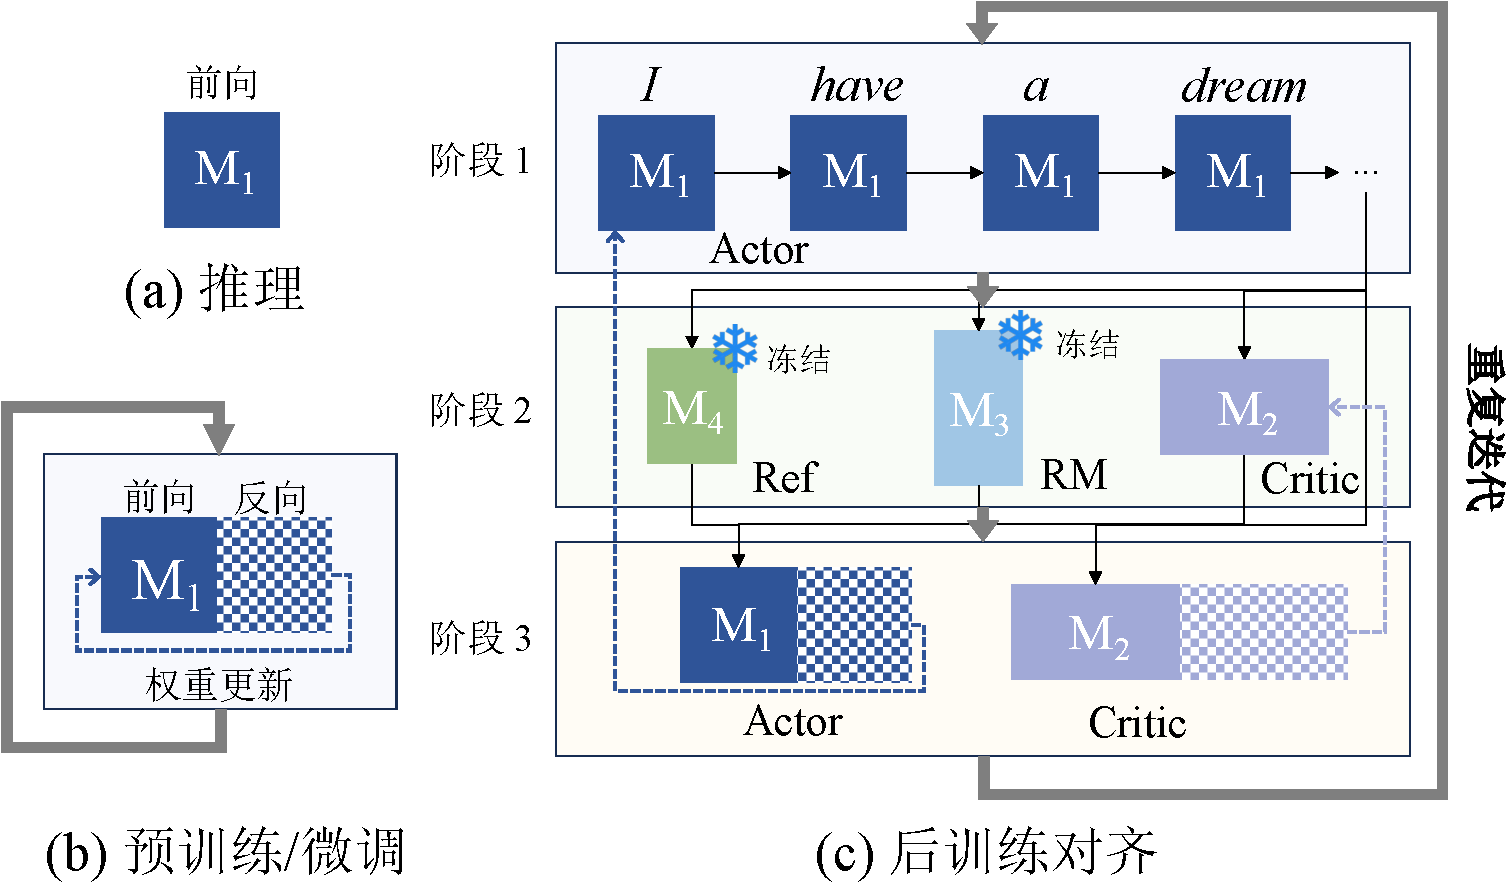
\includegraphics[width=0.7\linewidth, keepaspectratio]{figures/puzzle/1-intro-aligning-crop.pdf}
    % }
    \caption{推理、预训练、人工智能后训练对齐过程示意图}
    \label{fig:intro-aligning}
\end{figure}


大语言模型对齐的范式与现有人工智能系统所针对的标准全参数微调或预训练方法存在显著差异。
\Cref{fig:intro-aligning}以大语言模型对齐中公认的标准算法 PPO 为例,来说明推理、典型微调(或预训练)和对齐这几种范式之间的区别。
在微调过程中(如\Cref{fig:intro-aligning}(b)所示),仅需单个模型;而在对齐过程中(如\Cref{fig:intro-aligning}(c)所示),则需要多个模型,包括 Actor、Critic、Reference 和 Reward 模型。
根据模型的工作负载特征(推理或微调)以及它们之间的数据依赖关系,该范式可分为多个阶段,且不同模型之间的数据依赖仅存在于阶段之间。
后文将模型的工作负载和模型本身统称为上下文。 
本研究观察到,当前大语言模型对齐的标准方法具有以下不同特点: 

\begin{itemize}
    \item 
    \textbf{异构模型和工作负载}:
    PPO 等对齐方法涉及多种模型的协同参与,从而导致异构性。
    这种异构性源于两个方面:模型结构和工作负载。
    首先,不同模型的参数数量和结构存在显著差异;其次,对齐过程还引入了多样化的工作负载,如解码、推理和训练。
    因此,这些异构上下文使得对齐过程比标准微调更为复杂。 

    \item 
    \textbf{频繁的上下文切换}:
    整个对齐过程涉及以循环方式执行不同模型的不同工作负载(上下文),从而导致频繁的上下文切换。
    上下文切换不仅发生在阶段之间,也发生在阶段内部,例如当一个阶段内的多个模型按顺序执行时。
    如此频繁的切换会引入大量开销,包括模型重新加载、参数更新、数据传输等。
    例如,DeepSpeed-Chat 在收集更新后的参数时会产生 12.43\% 的开销。 
\end{itemize}


目前,研究人员已提出大量人工智能系统以应对推理和训练等不同复杂场景。
然而,这些现有系统对于后训练对齐场景,存在以下两个局限性: 

\begin{itemize}
    \item
    \textbf{仅专注于单个模型}:
    现有研究 \cite{liaman2022alpa,narayanan2019pipedream,narayanan2021megatronv2,kwon2023vllm}专注于为单个模型优化算子、计算图和并行执行计划,但忽略了涉及多个模型协同训练的场景,错失了进行细粒度跨模型优化的机会。 
    \item
    \textbf{忽视模型中的多样化工作负载}:
    现有的推理 \cite{zhuohan2023alpaserve,kwon2023vllm,yu2022orca} 和训练系统 \cite{xiao2020antman,xiao2018gandiva} 为其模型维持固定的工作负载,在执行过程中不需要更改配置(如并行执行计划)。
    在这些系统中,没有充分考虑对齐过程中所需的频繁上下文切换,从而导致了巨大且难以接受的成本。 
\end{itemize}

因此,本研究认为在大语言模型对齐中,异构上下文之间的高效切换是一项关键挑战,并且这仍是一个有待解决的研究问题。 

为应对这些挑战,本研究提出了一个高效大语言模型对齐系统 PUZZLE。
该系统将模型上下文视为核心要素,研究了大语言模型对齐过程中的模型编排,充分考虑了其中涉及的异构上下文,并利用异构上下文之间的相似性来实现轻量级、流畅的上下文切换。
具体而言,为了有效处理对齐过程中的异构上下文特性,PUZZLE 采用二维方法,同时考虑阶段内和阶段间的上下文切换。
在每个阶段内,本研究通过探索不同上下文之间的亲和性,并利用时间共享策略实现计算重叠,从而将切换成本降至最低。
此外,为了减少阶段之间的切换开销,本研究制定了基于相似性的方案,以找到通信成本最小的最优阶段间上下文切换方案。
本研究在配备多达 32 个 GPU 的不同集群上对 PUZZLE 进行了评估,结果表明,与最先进的 RLHF 训练系统 DeepSpeed-Chat\cite{yao2023deepspeedchat}相比,PUZZLE 在端到端训练中的加速比最高可达 2.12 倍。 
总之,本研究做出了以下贡献: 

1. 从人工智能后训练对齐问题中抽象出上下文的关键概念,并定位上下文切换为关键性能瓶颈之一。 

2. 提出了一种时间共享策略,用于探索阶段内不同上下文之间的亲和性,并将其整合到混合方案中,以降低阶段内上下文切换开销。 

3. 制定了基于相似性的方案,以找到通信成本最小的最优阶段间上下文切换方案。 

4. 基于上述技术实现了一个端到端的后训练对齐系统PUZZLE,与现有最先进的系统相比,实现了高达 2.12 倍的加速。 


\section{研究动机}
如前所述,在大语言模型对齐过程中,异构上下文之间的高效切换(包括阶段内上下文切换和阶段间上下文切换)是一项关键挑战。
本节重点阐述实现高效阶段内和阶段间切换的研究动机与机会。

(1) \textbf{阶段内上下文切换}:大语言模型对齐过程中的多个模型和工作负载涉及异构上下文,并且由于一个阶段内的这些异构上下文之间不存在数据依赖关系,因此可以采用多模型并行执行方案进行执行。
本研究观察到,所选方案在并行执行过程中常常出现大量空闲时间,这主要归因于以下原因:异构上下文之间存在显著差异,即便采用最优的方案组合,仍会产生空闲时间。
本研究的动机在于通过细粒度调度探索上下文之间的亲和性,目标是在相对最优的方案中实施时间共享策略,以最大限度地减少空闲时间。 

(2)	\textbf{阶段间上下文切换}:在对齐过程中,同一模型的上下文可能具有不同的工作负载,例如生成(解码)和训练阶段。
工作负载特征的差异导致最优并行执行方案完全不同。
例如,\Cref{fig:motiv2}(a)展示了 Llama-7B 模型在不同并行执行方案下生成和训练的性能表现。
为清晰起见,本研究省略了数据并行维度(图中的数据并行维度固定为 1),其中(P, T)分别表示流水线并行和张量并行维度。
此外,为了在不同阶段实现同一模型的最佳性能,还需要仔细考虑不同方案之间的参数重组开销,这是阶段间上下文切换成本的主要来源。
\Cref{fig:motiv2}(b)展示了不同方案下的切换成本,本研究观察到,对于相似性较高的方案,它们之间的切换成本要低得多。 

\begin{figure}[ht]
    \centering
    % \resizebox{0.75\linewidth}{!}{
    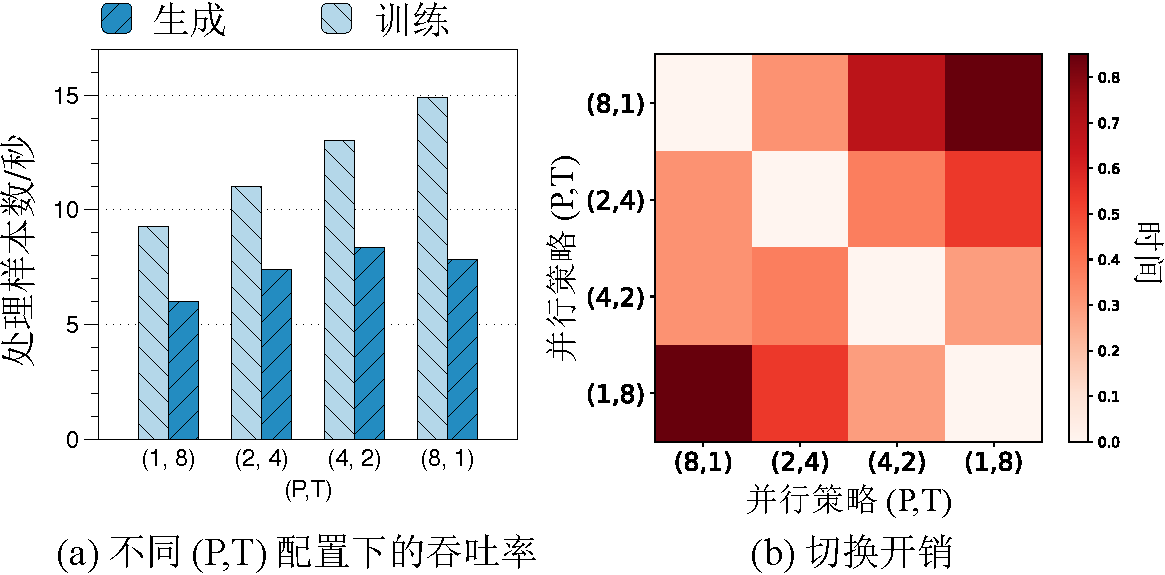
\includegraphics[width=0.7\linewidth, keepaspectratio]{figures/puzzle/2-bg-pic2-crop.pdf}
    % }
    % \vspace{-0.8cm}
    % \setlength{\abovecaptionskip}{0.cm}
    % \setlength{\abovecaptionskip}{0.cm}
    \setlength{\belowdisplayskip}{4pt}
    \caption{不同并行策略下的阶段性能对比}
    \label{fig:motiv2}
\end{figure}

\section{系统设计}
本研究提出了一个用于大语言模型的高效对齐系统PUZZLE,其名称源于每个异构上下文都类似于拼图的一块,本研究的目标是将这些 “拼图块” 合理布局,并在系统中高效执行。 

\Cref{fig:overview}展示了 PUZZLE 的系统概览。
该系统的核心概念基于对齐过程中遇到的独特异构模型和工作负载属性(本文中称为上下文)。
由于异构上下文特性,需要在阶段内和阶段间频繁切换,这会导致开销增加。
PUZZLE 旨在通过挖掘阶段内和阶段间过程中的潜在机会,降低此开销并提升系统效率。 

在\Cref{puzzle:section:intra-stage}中,本研究通过探索不同上下文之间的亲和性,并利用时间共享策略实现计算重叠,从而最小化阶段内切换成本;在\Cref{puzzle:section:inter-stage}中,本研究介绍阶段间上下文切换,通过找到具有高度相似性且通信成本最小的最优并行执行方案,来降低阶段间切换成本。 

\begin{figure}[h]
    \centering
    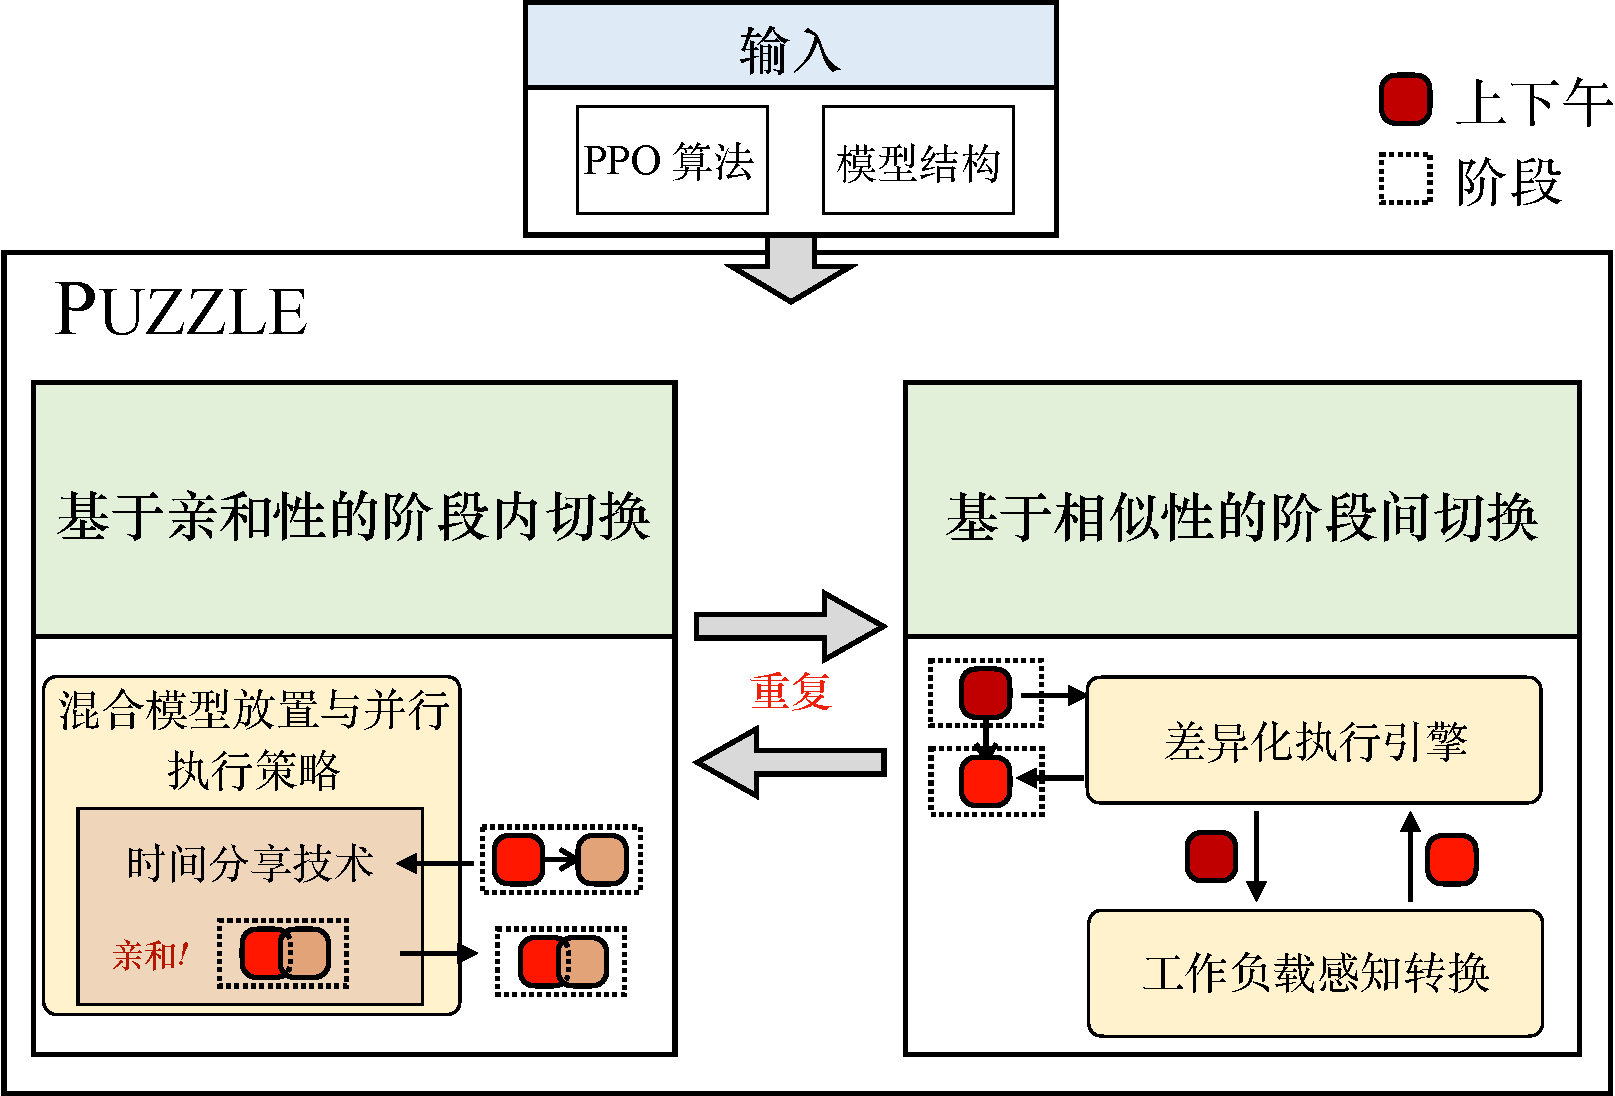
\includegraphics[width=0.7\linewidth]{figures/puzzle/3-overview-crop.pdf}
    \caption{PUZZLE系统设计}
    \label{fig:overview}
\end{figure}


\section{基于亲和性的阶段内切换}
 \label{puzzle:section:intra-stage}
尽管现有的并行执行技术效率较高,但在大语言模型对齐方面仍有提升空间,尤其是在并行执行方案中的上下文切换过程中存在空闲时间。
对齐过程中的异构上下文可划分为不同阶段,本研究发现,对每个阶段内的上下文进行编排能够显著提升阶段内上下文切换效率。

本节介绍基于亲和性的阶段内切换技术,该技术应用于 PUZZLE,用于探索不同上下文之间的布局和执行方案。
首先,本研究分析阶段内上下文切换的开销和潜在机会,并引入新的时间共享切换方案以促进上下文协作;最后,将所有现有方法相结合,形成多样化的布局和执行策略空间,即混合方案。

\subsection{布局和执行方案的机会}
尽管此前已有研究探索了对模型布局和执行的支持,但一个普遍的局限在于缺乏对上下文之间协作的关注,在对齐过程的同一阶段内,计算效率仍有很大的提升空间。
本研究首先分析阶段内上下文切换的开销和潜在机会。 

\textbf{开销的定义}:首先,本研究分析阶段内上下文切换可能引入的开销类型。
对于不共享资源的布局和执行方案,它们之间无需进行上下文切换,因此不会引入开销;然而,在资源共享的场景中,上下文按顺序执行,从而会引入开销。 

\textbf{潜在机会}:本研究观察到两个上下文可以实现重叠,
这是因为 PUZZLE 采用了混合并行化,包括张量并行、数据并行和流水线并行。
本研究主要关注流水线并行带来的开销,通常称为 “流水线气泡”。
这种开销会导致在流水线填满之前或接近完成时,某些设备处于空闲状态,进而影响整体吞吐量。
此类 “流水线气泡” 可能导致不必要的计算,尤其是在存在依赖关系的场景中。 

\textbf{基于亲和性的方法}:在涉及众多模型参与的对齐过程中,每个模型的并行策略可能存在显著差异。
然而,根据为每个模型选择的并行策略,本研究可以探索它们之间的亲和性。
在此,亲和性是指当两种并行策略高度相似时,计算过程能够有效重叠。 


\begin{figure}[ht]
    \centering
    % \resizebox{\linewidth}{!}{
    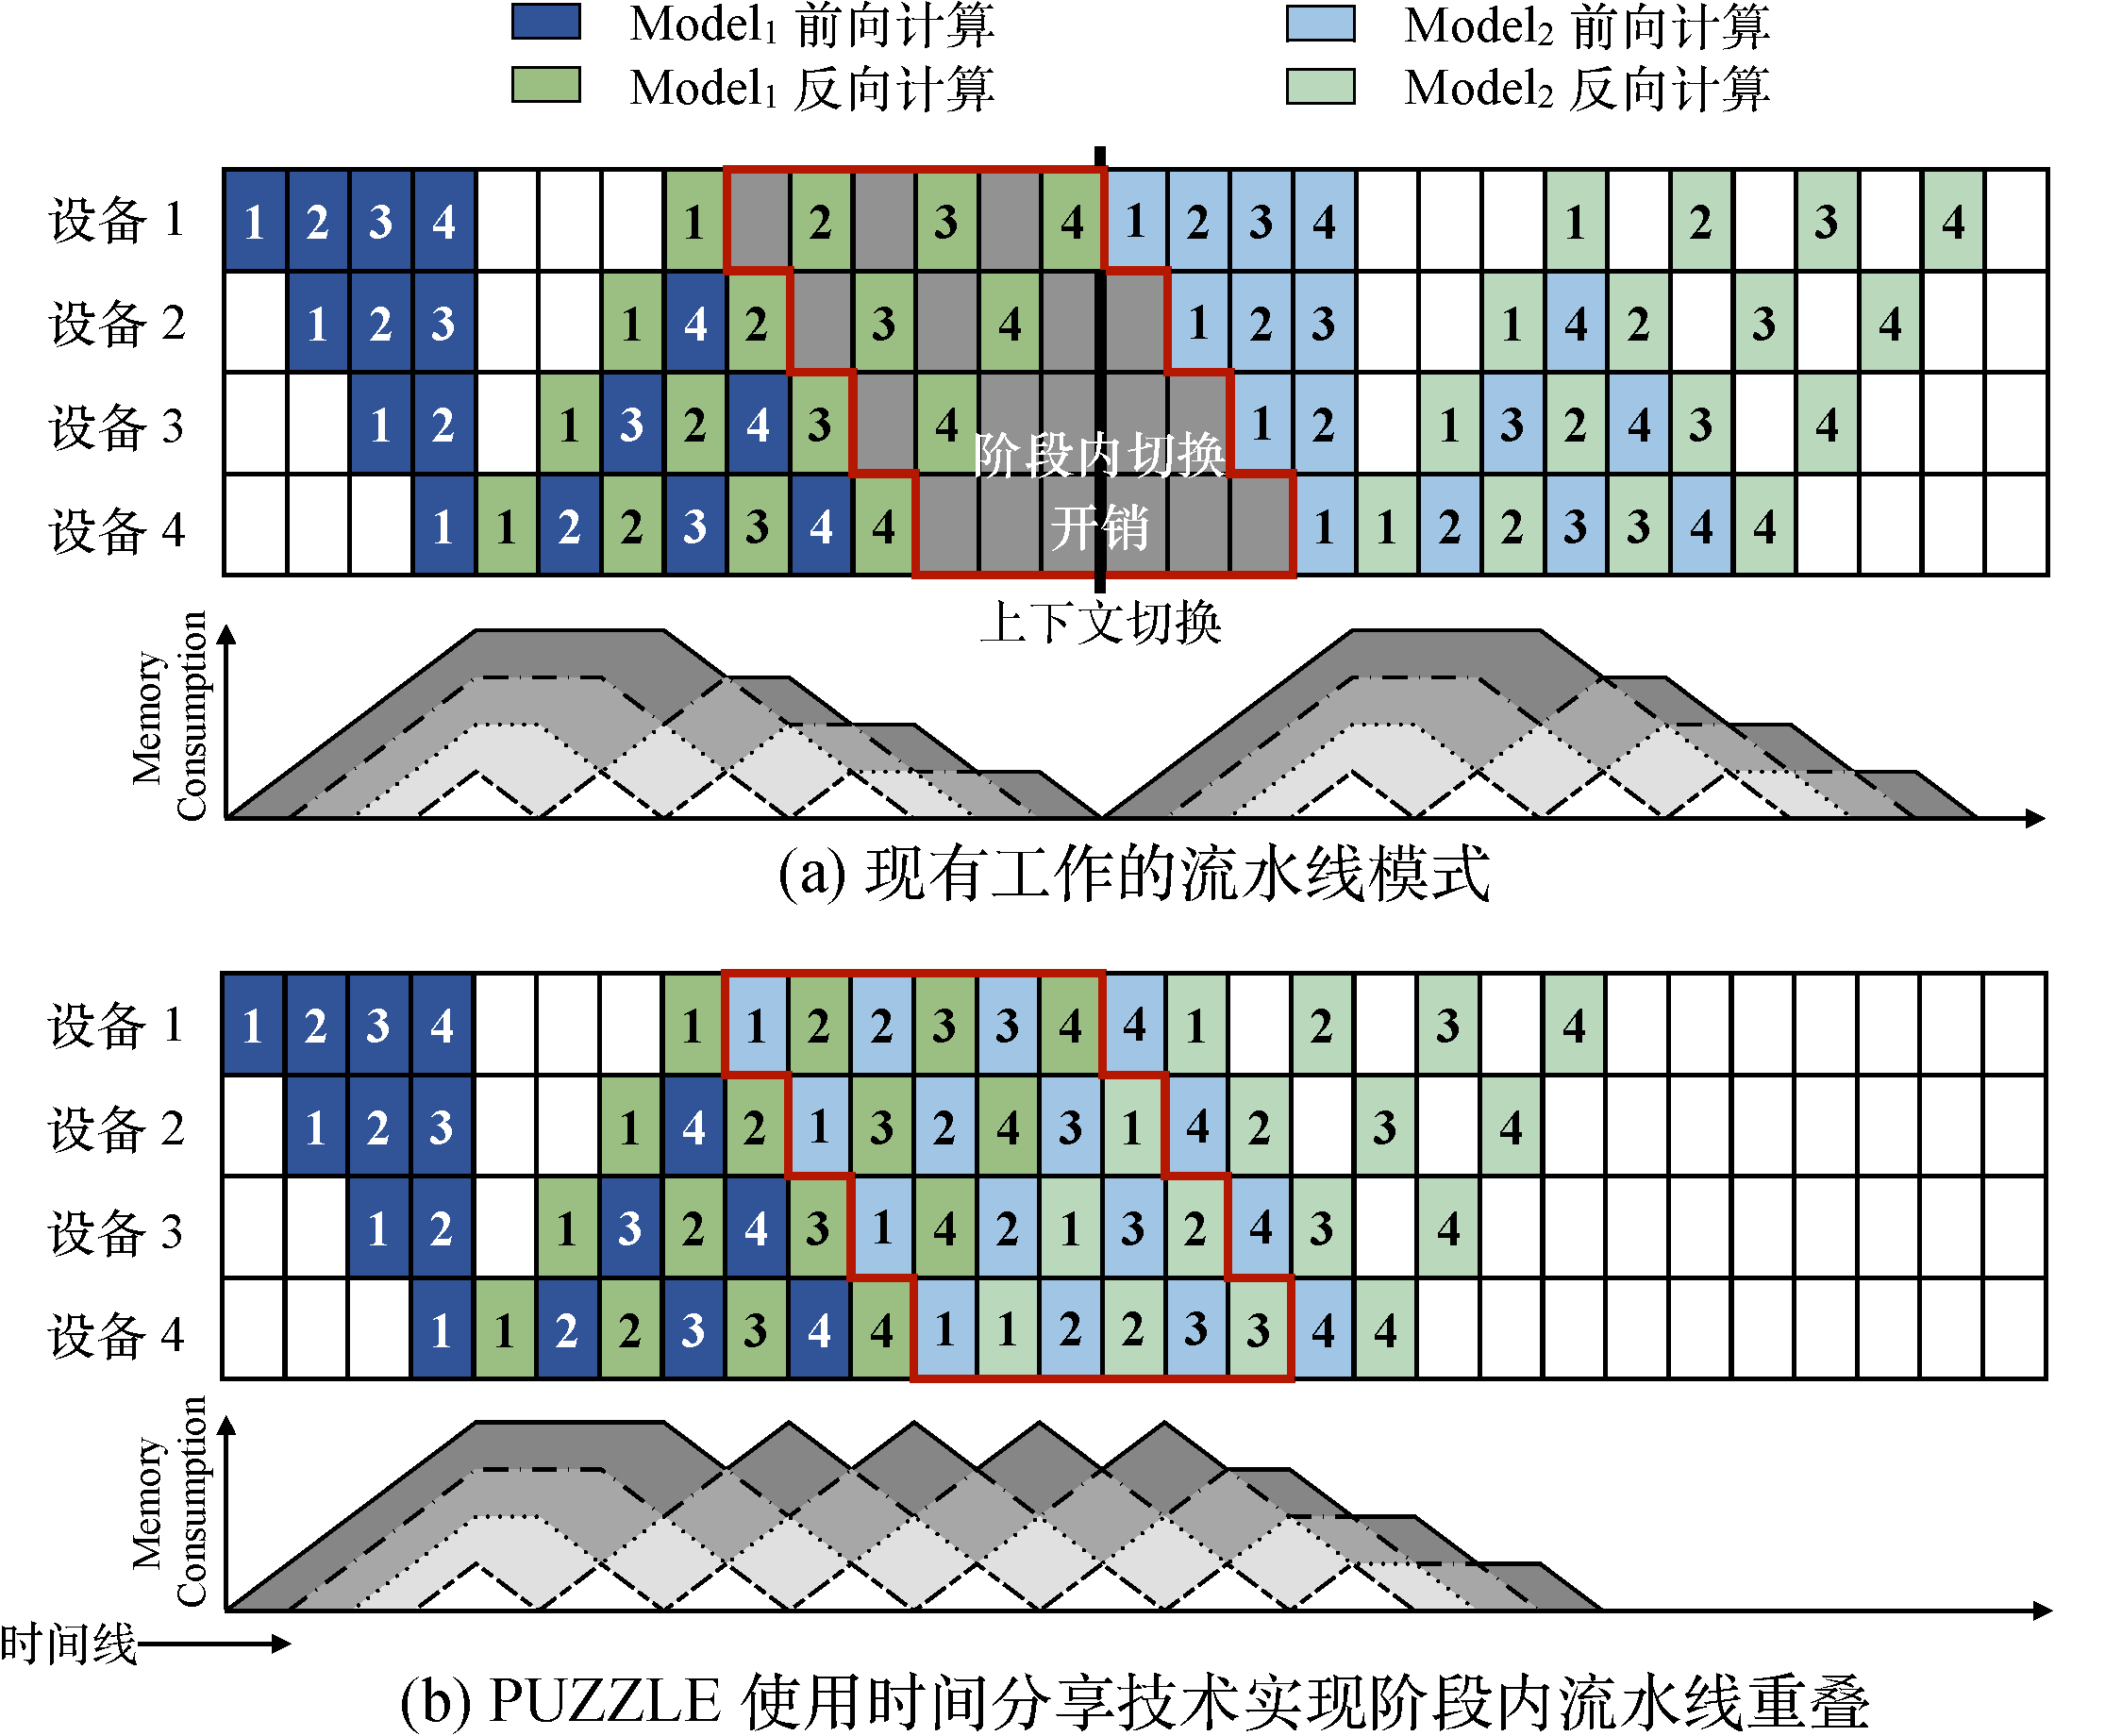
\includegraphics[width=0.8\linewidth]{figures/puzzle/4-intra-stage-context-switch-crop.pdf}
    % }
    \caption{阶段内流水线优化示意图
    }
    \label{fig:overlapping_example}
\end{figure}

\subsection{时间共享切换方案}
本节介绍一种新的主要执行方案,该方案旨在降低阶段内上下文切换的开销,实现共享相同资源的不同上下文之间的细粒度时间共享。
PUZZLE 在对齐过程中采用这种时间共享技术来探索上下文协作。 
本研究首先回顾训练两个模型 A 和 B 的传统策略,其执行顺序为顺序执行。
\Cref{fig:overlapping_example}(a)展示了两个模型的训练过程,每个模型被划分为四个部分,每个部分分配给一个设备,形成四层流水线,工作流程还包括四个微批次,两个模型按顺序执行。
然而,如\Cref{fig:overlapping_example}(a)中的灰色框所示,在两次上下文切换之间会产生大量 “气泡”,在这些空闲时间段内,设备处于闲置状态。因此,这种场景存在显著的优化空间,尤其是对于无依赖关系的任务执行。 

\Cref{fig:overlapping_example}(b)展示了时间共享技术的一个示例。
通过将后续训练任务与前一个任务相结合,可以有效利用前一个任务的空闲时间。
这种时间共享技术类似于操作系统中的进程并发,由于这些任务之间不存在依赖关系,因此可以并发执行。
例如,在模型 B 的第一个微批次前向传播在模型 A 的第一个微批次反向传播之后立即执行,此时执行时间为 9,而不是延迟到 15。
此外,图中所示的调度类似于在单个模型中完成八个微批次的训练。 

\textbf{理论加速比}:在\Cref{fig:overlapping_example}(b)中,模型 2 的第一个微批次前向传播在模型 1 的第一个微批次反向传播之后开始,此时模型 1 处于冷却阶段,模型 2 处于预热阶段。
设\(T^{f}\)表示每个前向传播的时间,\(T^{b}\)表示每个反向传播的时间,\(T^{idle}\)表示空闲时间。
在顺序执行中,总时间 \(T_{seq} = 4(T^{f} + T^{b}) + T^{idle}\);而在时间共享执行中,总时间 \(T_{ts} = 4(T^{f} + T^{b}) - T^{idle}\)。

% 因此,理论加速比 \(S = \frac{T_{seq}}{T_{ts}}=\frac{4(T^{f} + T^{b}) + T^{idle}}{4(T^{f} + T^{b}) - T^{idle}}\)。
% 可以看出,空闲时间 \(T^{idle}\) 越大,加速比 \(S\) 越高。


然而,由于在LLM对齐过程中存在异构的上下文,它们的执行时间各不相同。
为了更全面地理解细粒度时间共享技术所带来的加速效果,本研究进行了理论分析。
回顾时间共享技术的本质,它通过在两个上下文之间进行交错执行,使得较短持续时间的上下文能够减少预热和冷却阶段的时间开销。
因此,在假设微批次数量为 $N_B$ 的情况下,理论上可以获得的加速比可以表示为:


\begin{equation}
\begin{split}
\label{equation:theoretical-speedup}
% &理论加速比 \\
% &\frac{(N_{B}+P-1)(T^f_1+T^b_1+T^f_2+T^b_2)}{N_{B}(T^f_1+T^b_1+T^f_2+T^b_2)+(P-1)\max\limits_{k\in\{1,2\}}{(T^f_k+T^b_k)}}
&\frac{(N_{B}+P-1)\sum_{k\in\{1,2\}}(T^f_k+T^b_k)}{N_{B}\sum_{k\in\{1,2\}}(T^f_k+T^b_k)+(P-1)\max\limits_{k\in\{1,2\}}{(T^f_k+T^b_k)}}
% \Sigma_{i=1}
\end{split}
\end{equation}

其中,
$P$ 表示并行处理的模型上下文数量(例如 2),
$T^f_k$ 和 $T^b_k$ 分别表示第 $k$ 个模型的前向传播和反向传播时间,
分子代表顺序执行两个模型时的总时间(包括预热和冷却),
分母代表时间共享交错执行的实际总时间。



\textbf{内存消耗分析}:
与原始的顺序执行版本相比,本研究的新执行计划在峰值内存消耗上保持一致。
这是因为在PUZZLE中采用了1F1B同步流水线模式,其内存使用遵循如下规律:  
在前向传播阶段保留激活张量时达到峰值,随后在完成反向传播后逐渐下降。

如\Cref{fig:overlapping_example}(a) 所示,内存使用从谷值上升到峰值,再回落到谷值的过程重复了两次,对应两个连续模型的顺序执行。  
而以 Device1 为例,在 Model$_1$ 的第一个微批次前向传播激活张量被释放后,系统立即开始 Model$_2$ 的第一个微批次前向传播,如\Cref{fig:overlapping_example}(b) 所示。  
这种时间共享方式并未增加内存压力,反而优化了设备的计算资源利用率,实现了更高的吞吐效率。


% \textbf{实现方面}:为了实现时间共享切换方案,本研究需要解决两个关键问题:何时进行上下文切换以及如何进行上下文切换。
% (1) \textit{何时切换}:在流水线并行中,每个设备负责模型的一个阶段,并且在每个微批次中,设备需要等待上一个阶段的设备完成计算并将数据传输过来后才能开始计算。
% 因此,本研究可以利用设备等待数据的时间来执行其他上下文的计算。
% 具体来说,当一个设备完成了当前上下文的前向传播并且正在等待上一个阶段的设备传输反向传播的数据时,本研究可以在这个设备上启动另一个上下文的前向传播。
% 这样,两个上下文的计算就可以在时间上重叠,从而提高计算资源的利用率。
% (2) \textit{如何切换}:在进行上下文切换时,本研究需要确保两个上下文之间的数据不会相互干扰。
% 为此,本研究为每个上下文分配独立的内存空间,并且在切换上下文时,保存当前上下文的计算状态(如中间变量、梯度等),并加载下一个上下文的计算状态。
% 这样,每个上下文的计算都可以独立进行,不会受到其他上下文的影响。


\begin{figure}[ht]
    \centering
    % \resizebox{\linewidth}{!}{
    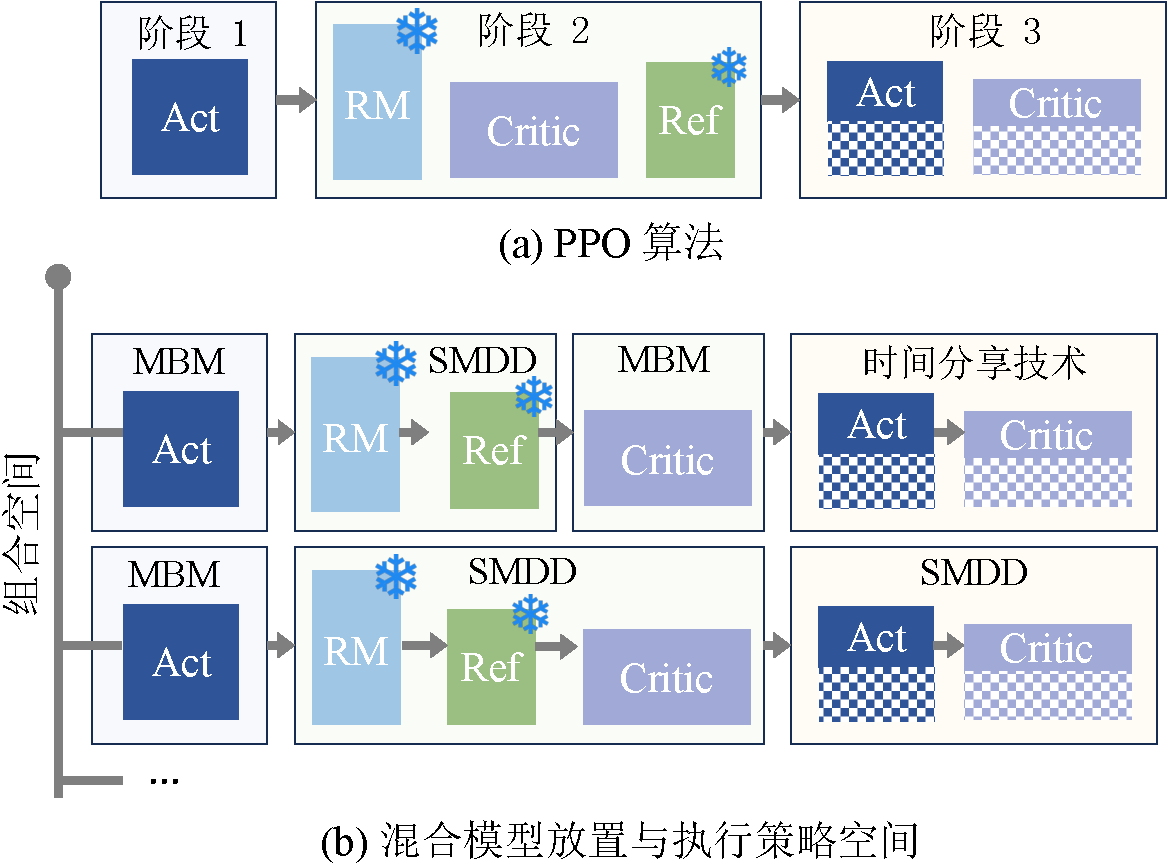
\includegraphics[width=0.7\linewidth]{figures/puzzle/4-hybrid-plan-2-crop.pdf}
    % }
    % \vspace{-0.8cm}
    \caption{不同混合放置与执行计划示意图}
    \label{fig:hybrid-plan}
\end{figure}

\subsection{混合放置与执行计划}
\label{subsection:intra-stage-hybrid-plan}

最后,通过整合所有现有方法,本研究丰富了模型放置与并行执行计划的组合空间,称之为混合计划。  
在混合计划中,对齐过程可以根据每个阶段的工作负载特性划分为多个阶段组,而这些阶段组还可以进一步划分为子阶段组。  
每个子阶段可以基于其特性选择合适的放置和执行计划。  
不同子阶段组之间的执行计划是顺序执行的,这意味着每个子阶段组可以占用全部计算资源来执行该阶段组的功能。  
对于需要细粒度调度的阶段组,应保持并行执行计划的一致性。  
\Cref{fig:hybrid-plan} 提供了一些简单示例,用于演示混合布局与执行计划的工作原理。

如\Cref{fig:hybrid-plan}(a) 所示,整个对齐过程可以划分为三个阶段,每个阶段都依赖于前一个阶段的结果。  
不同的方框代表不同的模型,某些模型可能同时存在于多个阶段中。  
正如之前所提到的,阶段组可以被划分为更小的子阶段组,每个子阶段组可以选择不同的放置和执行计划。  
\Cref{fig:hybrid-plan}(b) 展示了两种可能的执行方案:

(1) 在第一种方案中,单一模型阶段组等同于采用 MBM(Multiple Batch, Multiple Model)计划,  
而 \texttt{Act} 和 \texttt{Critic} 阶段组则采用细粒度的时间共享计划(fine-grained time-sharing plan)。

(2) 在第二种方案中,类似于调度器的方式,每个阶段组基本采用 SMDD(Single Model, Dedicated Device)计划,即阶段组内的每个模型独占计算资源进行执行。



% \subsection{混合方案}
% 虽然时间共享切换方案能够有效利用空闲时间,提高计算资源的利用率,但它并不能完全消除上下文切换的开销。
% 此外,不同的上下文可能具有不同的计算特性和资源需求,单一的时间共享切换方案可能无法适用于所有情况。
% 因此,本研究提出了一种混合方案,将时间共享切换方案与其他现有的布局和执行方案相结合,以提供更灵活和高效的上下文管理方式。
% 具体来说,混合方案包括以下几个步骤:

% (1) \textbf{方案选择}:根据每个上下文的计算特性(如计算密集型或通信密集型)和资源需求(如内存需求、计算能力需求等),选择合适的布局和执行方案。例如,对于计算密集型的上下文,本研究可以选择张量并行方案,以充分利用设备的计算能力;对于通信密集型的上下文,本研究可以选择数据并行方案,以减少通信开销。

% (2) \textbf{时间共享调度}:对于选择了相同资源的上下文,本研究采用时间共享切换方案进行调度,以实现计算重叠,减少空闲时间。在时间共享调度过程中,本研究根据上下文之间的亲和性,确定它们的执行顺序和时间分配,以最大化计算资源的利用率。

% (3) \textbf{动态调整}:在执行过程中,本研究实时监测系统的资源使用情况和上下文的执行状态,并根据监测结果动态调整布局和执行方案。例如,如果某个上下文的执行速度较慢,导致其他上下文等待时间过长,本研究可以调整该上下文的并行策略或重新分配资源,以提高其执行速度。
% 通过混合方案,本研究可以根据不同上下文的特点和系统的运行状态,灵活地选择和调整布局和执行方案,从而有效地降低阶段内上下文切换的开销,提高大语言模型对齐的效率。


% \section{基于相似性的阶段间切换}
% 在大语言模型对齐过程中,阶段间上下文切换同样会带来显著的开销,主要源于不同阶段中同一模型的工作负载差异导致的最优并行执行方案不同,以及方案切换时的参数重组。为降低这些开销,本研究提出基于相似性的阶段间切换策略,旨在找到通信成本最小的最优并行执行方案。

% \subsection{并行执行方案的相似性度量}
% 为找到最优的阶段间切换方案,首先需要定义一种度量方式来评估不同并行执行方案之间的相似性。本研究从两个维度来考虑方案的相似性:参数布局相似性和通信模式相似性。
% 参数布局相似性:大语言模型的参数在不同并行执行方案下的布局方式对切换成本有重要影响。本研究通过比较不同方案中参数在设备间的分布情况来衡量参数布局相似性。具体而言,对于每个模型的参数,本研究计算在两种方案下参数在相同设备上的比例。假设模型有 \(N\) 个参数,在方案 \(A\) 和方案 \(B\) 下,有 \(n\) 个参数位于相同的设备上,则参数布局相似性得分 \(S_{p} = \frac{n}{N}
% \)。得分越高,表明两种方案的参数布局越相似,在切换时需要进行的参数重组操作就越少,从而降低切换成本。
% 通信模式相似性:不同的并行执行方案会导致不同的通信模式,包括通信的设备对、通信的数据量和通信的频率等。本研究通过分析通信模式的这些要素来评估通信模式相似性。具体方法是,构建每个方案的通信矩阵,矩阵中的元素表示设备之间的通信关系和数据量。然后,计算两个通信矩阵之间的相似度。例如,可以使用余弦相似度来衡量两个通信矩阵的相似程度,设两个通信矩阵为 \(C_{A}\) 和 \(C_{B}\),则通信模式相似性得分 \(S_{c} = \frac{C_{A} \cdot C_{B}}{\vert\vert C_{A}\vert\vert \vert\vert C_{B}\vert\vert}\)。得分越高,说明两种方案的通信模式越相似,在切换时可以减少通信协议的重新配置和数据传输的调整,进而降低通信开销。
% 综合参数布局相似性和通信模式相似性,本研究得到并行执行方案的总体相似性得分 \(S = \alpha S_{p} + (1 - \alpha) S_{c}\),其中 \(\alpha\) 是一个权重系数,用于平衡参数布局相似性和通信模式相似性的重要程度。通过实验,本研究可以确定最优的 \(\alpha\) 值,以使得总体相似性得分能够最准确地反映方案切换成本。

% \subsection{最优方案搜索}
% 在定义了相似性度量后,本研究需要在所有可能的并行执行方案中搜索最优方案,以实现最小的阶段间上下文切换成本。由于可能的方案数量较多,穷举搜索是不可行的,因此本研究采用启发式搜索算法。
% 本研究从当前阶段的并行执行方案出发,通过对方案进行小的调整来生成候选方案。例如,可以改变流水线并行的阶段划分、调整张量并行的维度或者修改数据并行的分组方式等。对于每个候选方案,本研究计算其与下一阶段目标方案的相似性得分,并评估切换到该候选方案所需的成本,包括参数重组成本和通信成本。成本评估可以通过模拟方案切换过程,计算参数传输量、设备间通信次数和时间等指标来实现。
% 然后,本研究选择相似性得分最高且切换成本最低的候选方案作为下一阶段的执行方案。为了避免陷入局部最优解,本研究还引入了随机搜索和模拟退火等策略,在一定程度上探索更广泛的方案空间。通过不断迭代搜索过程,本研究能够找到接近最优的阶段间上下文切换方案,从而有效降低阶段间切换开销,提高大语言模型对齐的整体效率。

\section {基于相似性的阶段间切换}
\label {puzzle:section:inter-stage}

对齐过程需要自适应并行执行计划,以根据当前计算特性维持阶段间的最优性能。
然而,在运行时调整并行执行计划并非易事,尤其是在混合并行场景中——不同计划会基于并行度在设备间分配参数,导致每层的层数和参数数量发生变化。
因此,运行时转换的主要挑战在于:在考虑参数分布的同时,以最小开销实现计划的高效切换。  

本节介绍基于相似性的阶段间切换技术,它在兼顾切换开销的同时最大化性能。
\Cref{fig:inter-stage-section-overview} 展示了 PUZZLE 中阶段间切换的示例。
PUZZLE 通过相似性准则寻找通信成本最低的最优并行执行计划,具体包括:
首先介绍用于为同一模型执行不同工作负载的差异化执行引擎;
其次引入以最小通信成本转换执行计划的工作负载感知转换;
最后概述阶段间切换目标并提出面向相似性的计划设计。  


\subsection{差异化执行引擎}
\label{subsection:inter-stage-diff-exec-engine}

在大语言模型对齐中,同一模型可能负责不同类型的工作负载,称为差异化工作负载。
例如,\texttt{Actor} 模型需要同时处理生成和微调任务,分别代表两个阶段的上下文。
但这两种工作负载表现出不同的计算特性和需求。
因此,本研究设计了差异化执行引擎,以适应模型在不同阶段的可变工作负载。
如\Cref{fig:inter-stage-section-overview} 所示,在模型执行下一阶段(如从微调切换到生成)之前,需要通过工作负载感知转换采用更高效的并行执行计划,同时最小化通信成本。
转换完成后,差异化执行引擎基于转换后的阶段执行工作负载。  


\subsection{工作负载感知转换}
\label{subsection:inter-stage-workload-aware-trans-engine}

以下介绍 PUZZLE 中使用的工作负载感知转换,其设计目标是通过最小化通信成本实现高效的阶段间上下文切换,如\Cref{fig:inter-stage-section-overview} 所示。
根据之前的分析,从训练到生成的并行度转换涉及从较高的流水线并行度向较低的流水线并行度转变,该过程需要将原始层的参数与其他节点共享以形成张量并行组。
因此,本研究首先分析此类切换相关的通信流量,并引入相似性概念以识别通信成本最低的最优并行执行计划。  


\begin{figure}[t]
    \centering
    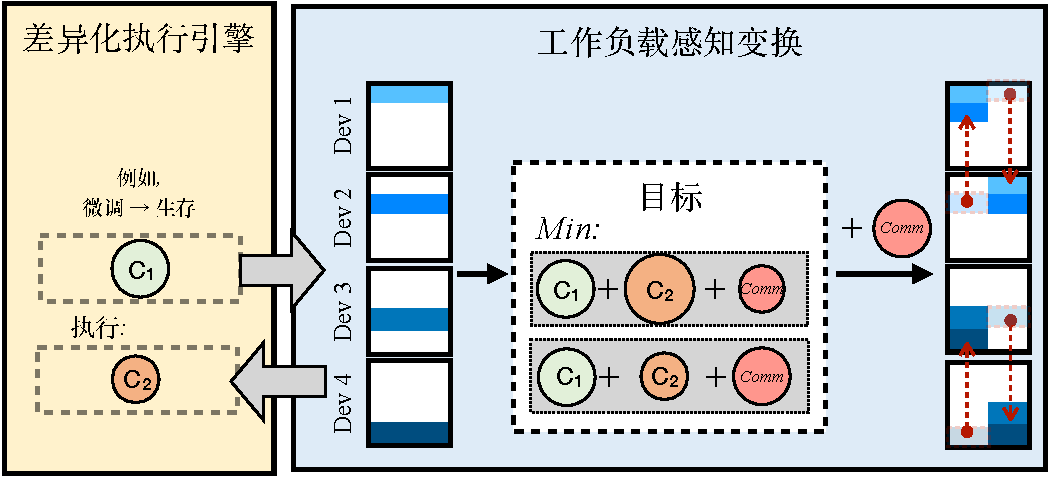
\includegraphics[width=0.75\linewidth]{figures/puzzle/5-inter-stage-section-overview-crop.pdf}
    % \vspace{-0.4cm}
    \caption{PUZZLE 中阶段间切换的示意图}
    \label{fig:inter-stage-section-overview}
\end{figure}


\textbf{通信量分析}:在 PUZZLE 中,混合并行(包括数据并行、张量并行和流水线并行)用于显著减少通信。下面本研究以混合精度训练为例,对此类通信减少进行分析。  
假设一个模型包含 $L$ 层,训练在 $N$ 个工作节点的集群上进行,$P$、$D$、$T$ 分别表示流水线并行、数据并行和张量并行的方式。每个设备需要广播的次数可由公式 $f_{P}=\frac{P_{src}}{P_{dst}}$ 确定。本研究使用\Cref{fig:inter-stage-section-overview} 中的具体示例说明该过程,其中 $(L,N)=(4,4)$,计划转换涉及从 $(P, D, T)=(4,1,1)$ 到 $(2,1,2)$ 的转变。需要注意的是,上述示例仅说明了 $D=1$ 的情况,而 PUZZLE 能够处理 $D>1$ 的情况。因此,在 PUZZLE 的单个训练步骤中,传输仅涉及 GPU 之间 $D-\frac{1}{f_{P}}$ 次参数复制。  


% \textbf{路由表生成}:PUZZLE 利用 \textit{路由表} 确定哪些工作节点需要广播数据以及哪些工作节点组需要接收数据。基于转换前后的并行执行计划,PUZZLE 能够生成相应的路由表。  
% 受数制转换的启发,本研究设计了路由表生成算法以生成计划转换的路由表。
% 在该算法中,$base$ 定义为三元组 $(P,D,T)$,表示 rank 遵循张量并行、数据并行和流水线并行的维度顺序。
% 例如,若 rank 为 3,在 $base_{1}=(4,1,1)$ 中对应 $(3,0,0)_{base_{1}}$,而在 $base_{2}=(2,1,2)$ 中对应 $(1,0,1)_{base_{2}}$。本研究使用函数 \textsc{GetIndex} 将 rank 转换为 $base$ 下的索引,使用函数 \textsc{GetRank} 还原为 rank。变量 $f_P$、$f_D$、$f_T$ 表示 $src$ 和 $dst$ 之间不同维度的比率。  

% 函数 \textsc{GetRoutingTBL} 生成需要从 $rank$ 向目标节点广播参数的路由表。在该函数中,首先将 $rank$ 转换为 $base_{src}$ 下的索引 $id_{src}$(\Cref{alg:line:get-index-in-tlb}),然后计算 $base_{dst}$ 下的对应索引 $id_{dst}$(\Cref{alg:line:calc-index}),最后使用 \textsc{GetRank} 获得 rank 编号。每个 $rank$ 对应 $f_P$ 个需要广播数据的目标节点。  


% \begin{algorithm}
% \caption{路由表生成}
% \begin{algorithmic}[1]
% \Function{GetIndex}{$r, base$} \Comment{$base$ 为 $(P,D,T$)} \label{alg:line:get-index}
%     \State $P, D, T \gets base$
%     \State \Return $(\frac{r}{D \times T} \bmod P,\frac{r}{T}\bmod D, r \bmod T)$
% \EndFunction

% \Function{GetRank}{$idx, base$} \label{alg:line:get-rank}
%     \State $P, D, T \gets base$
%     \State \Return $idx[0] \times D \times T + idx[1] \times T + idx[2]$
% \EndFunction

% \Function{GetRoutingTBL}{$rank, base_{src}, base_{dst}$} \label{alg:line:get-rttlb}
%     \State $TBL \gets \{rank:[\ ]\}$
%     \State $f_P, f_D, f_T \gets \Call{BitwiseDiv}{base_{src}, base_{dst}}$
%     \State $id_{src} \gets \Call{GetIndex}{rank, base_{src}}$ \label{alg:line:get-index-in-tlb}
%     \For{$i \gets 0$ to $f_P - 1$}
%         \State $id_{dst} \gets (\frac{id_{src}[0]}{f_P}, id_{src}[1], \frac{id_{src}[2]}{f_T} + i)$ \label{alg:line:calc-index}
%         \State 将 $\Call{GetRank}{id_{dst}, base_{dst}}$ 追加到 $TBL[rank]$
%     \EndFor
%     \State \Return $TBL$
% \EndFunction
% \end{algorithmic}
% \label{alg:rout-table-gen}
% \end{algorithm}


\textbf{异步权重转换}: 在对齐过程中,训练数据生成通常使用最新的参数,这些参数在优化步骤中更新。
此外,参数更新使用优化器状态和梯度执行,且这些更新之间没有依赖关系。因此,优化步骤和参数交换可以异步执行并交错进行。  
本研究通过双流调度最小化权重转换开销。在 PUZZLE 中,可训练参数被划分为 $n$ 个段,如 $P_1, P_2,\ldots,P_k$。
在每个部分优化步骤和参数更新之后,转换引擎将这些参数广播到其他设备,实现并行操作并减少端到端延迟。  


\subsection{基于相似性的计划}
\label{subsection:inter-stage-goal}

并行执行计划的转换使 PUZZLE 能够识别更高效的策略来执行差异化工作负载,尽管该过程会产生额外的通信成本。在本节中,本研究的目标是描述阶段间上下文切换的目标,特别关注以轻量级方式实现此过渡。  
假设目标是通过从计划 $i$ 切换到计划 $j$ 来实现从上下文 A 到上下文 B 的过渡。本研究将计划 $i$ 下上下文 A 的时间定义为 $T^A_i$,计划 $j$ 下上下文 B 的时间定义为 $T^B_j$,从计划 $i$ 切换到计划 $j$ 所需的时间表示为 $T_{ij}$。根据这些定义,阶段间切换的目标可表示为:  

\begin{equation}
    \label{equation:inter-stage-goal}
    \min_{i,j} T^A_i + T^B_j+T_{ij}
\end{equation}

然而,在并行执行计划中识别实现最小目标的最优解并非易事。如\Cref{fig:motiv2} 所示,当并行执行计划更相似时,开销往往更低。
这种“相似性”是根据元组 $(P_i,D_i,T_i)$ 和 $(P_j,D_j,T_j)$ 之间的距离定义的。  
因此,本研究为阶段间切换提出了一种 \textit{面向相似性} 的方法。
基于这些观察,本研究从计划 $i$ 的 $(P,D,T)$ 配置开始,逐步减小 $P$ 的大小并增加 $T$ 的大小,同时根据\Cref{equation:inter-stage-goal} 持续评估是否存在性能提升,重复该过程直至不再出现性能提升。


\section{实验评估}

\subsection{实验设置}  

实验平台方面,本研究在两个网络拓扑和带宽不同的典型集群上进行评估:  

(1) {\textit{\textbf{orion}}} 是一个包含 32 个 GPU 的集群,分布在四个工作节点。每个节点配备 8 张 NVIDIA A100-PCIe-80GB GPU,通过 PCIe 交换机连接到 2 个 CPU 插槽,并搭载 100 Gb/s Infiniband EDR 网络。  

(2) {\textit{\textbf{phoenix}}} 是另一个包含 32 个 GPU 的集群,同样分布在四个工作节点。每个节点配备 8 张 NVIDIA A100-SXM-80GB GPU,通过 NVLink 互联形成异构环结构(其中一半连接因绑定两条链路而具备双倍带宽),并使用 100 Gb/s Infiniband EDR 通信。与 PCIe 相比,NVLink 为 GPU 连接提供更高的通信吞吐量。  

\begin{table}[h]
\caption{模型配置规格}
\label{table:model-info}
\small
\centering
\begin{tabular}{lcccc}
\toprule
参数数量      & 350M  & 7B       & 13B       & 33B       \\ 
\midrule
层数         & 16    & 32       & 40        & 64        \\
隐藏层维度   & 512   & 4096     & 5120      & 6656      \\
中间层维度   & 11008 & 11008    & 13824     & 17920     \\ 
\bottomrule
\end{tabular}
\end{table}


评估模型方面,
本研究的实验部分主要关注近端策略优化(PPO)算法,它是现代大语言模型 RLHF 对齐中的主流技术。
本研究采用不同参数规模的 Llama 模型,包括 350M、7B、13B 和 33B,具体规格如\Cref{table:model-info} 所示。  
实验中 PPO 算法的超参数配置如下:PPO 轮次和滚动(rollout)批量大小均设为 1,提示序列长度和生成长度均为 256。
为适应 GPU 有限的内存容量,本研究在 DeepSpeed-Chat 的生成阶段配置了较低的张量并行度。  
数据集采用 DeepSpeed-Chat 的默认数据集 \texttt{Dahoas/rm-static},这是托管于 HuggingFace 的开源数据集,专为 RLHF 对齐大语言模型设计,通常用于训练有帮助且无害的助手模型。 






对比系统方面,
本研究将 PUZZLE 与最先进的 RLHF 训练框架 DeepSpeed-Chat\cite{yao2023deepspeedchat} 进行对比。在与 DeepSpeed-Chat 的对比测试中,使用其实现的混合引擎——可在训练和生成阶段切换并行策略:训练阶段采用 ZeRO stage 3\cite{rajbhandari2020zero},生成阶段采用张量并行。  


评估指标方面,  
端到端评估中,本研究测量对齐过程的样本吞吐量(定义为从开始到完成处理样本的速率,单位:样本/秒)。  

\begin{table}[h]
\caption{评估使用的 PPO 算法配置}
\label{table:end2end-config}
\small
\centering
\begin{tabular}{lccc}
\toprule
配置          & 批量大小   & GPU 数量 \\ 
\midrule
7B/350M      & 128        &  8      \\
7B/7B        & 256        &  16     \\
13B/350M     & 256        &  16     \\
13B/7B       & 256        &  16     \\
33B/7B       & 128        &  32     \\
\bottomrule
\end{tabular}
\end{table}



\begin{figure*}[t]
    \centering
    % \resizebox{\linewidth}{!}{
    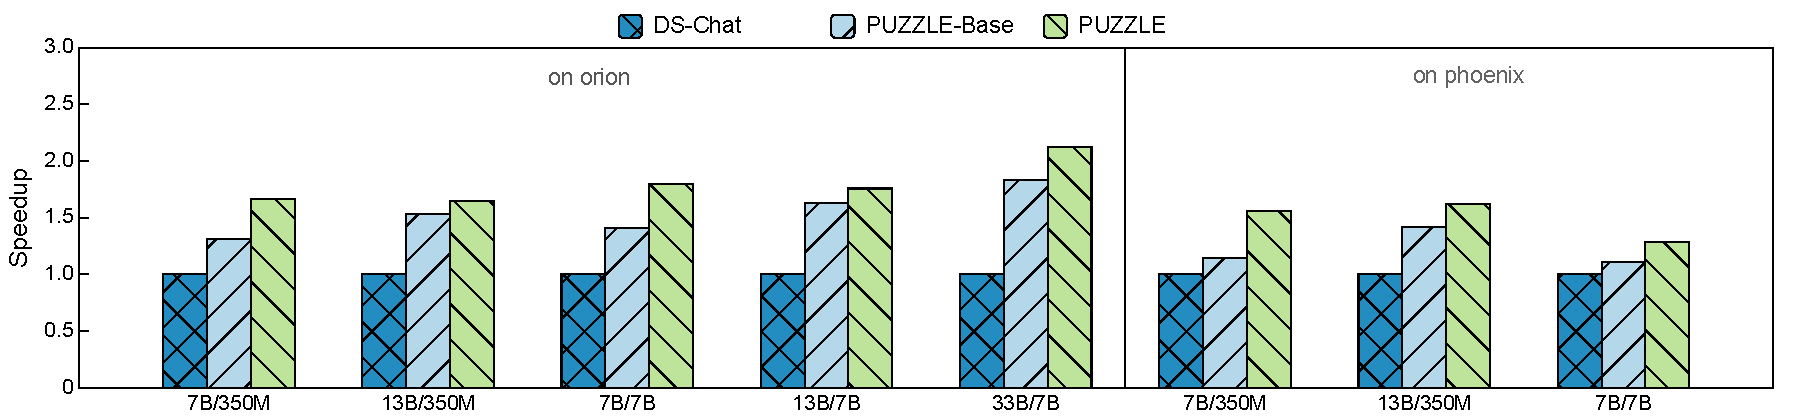
\includegraphics[width=\linewidth, keepaspectratio]{figures/puzzle/end2end.pdf}
    % }
    \vspace{-0.3cm}
    \caption{不同配置的端到端加速比}
    \label{fig:end2end}
\end{figure*}

\subsection{端到端性能}  

本研究在两个不同集群上评估了各种模型组合的端到端性能,评估配置详见\Cref{table:end2end-config}。
配置 X/Y 表示 PPO 中 Actor 和 Critic 模型的参数数量,参考模型和奖励模型分别与之对应。
这些配置采用弱扩展方式,批量大小随 GPU 数量增加而增大,但 33B/350M 配置因 GPU 内存限制做了调整。  

\Cref{fig:end2end} 展示了 PUZZLE 与使用混合引擎的 DeepSpeed-Chat 在两种集群配置下的端到端加速比对比,实验还纳入了仅使用流水线并行的 PUZZLE-Base。PUZZLE 在两个集群上分别实现了 1.83倍 和 1.50倍 的平均加速比。
对比 \textit{phoenix} 和 \textit{orion} 发现,PUZZLE 在 \textit{orion} 上加速比更高,原因是该集群 GPU 间带宽受限且节点内通信频繁,导致效率下降。
具体而言,生成阶段 DeepSpeed-Chat 为适应 GPU 内存限制选择更高的张量并行度,而 PUZZLE 通过为不同阶段选择最优混合并行执行计划并利用轻量级阶段间切换解决了这一问题。  

该实验进一步评估了仅使用流水线并行且无额外优化的 PUZZLE-Base,其解码阶段批量大小按流水线规模平均分配。
实验结果表明本研究系统的基线性能——显著优于 DeepSpeed-Chat。
此外,在 LLM 对齐的异构上下文中,仅依赖数据并行效率较低,因此需要同时考虑阶段内和阶段间优化以提升性能。  


\subsection{阶段内消融实验}  

本节分析阶段内上下文切换所使用的时间共享技术的有效性。
如\Cref{fig:intra-stage-ablation-study} 所示,本研究在两个集群上按\Cref{table:end2end-config} 的配置对比了不同配置下的阶段内性能,以不使用时间共享技术的配置作为基线。
显然,时间共享技术显著提升了阶段内上下文切换性能,减少了空闲时间,阶段内加速比最高达 1.12倍。图中还显示两个集群的加速比基本一致,表明时间共享技术在不同集群中均有效。
此外,在相似模型配置下,加速比更为显著,后续将对此进行分析。  

\begin{figure}[h]
     \centering
     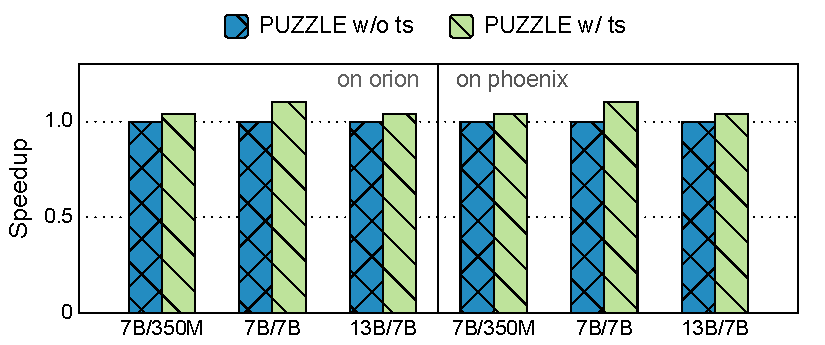
\includegraphics[width=0.65\linewidth]{figures/puzzle/intra-stage-ablation-study.pdf}
     \caption{时间分享技术性能分析} 
     \label{fig:intra-stage-ablation-study}
\end{figure}


\Cref{fig:intra-stage-theoretical} 展示了 PUZZLE 在各种配置和批量大小下相对于理论加速比(使用\Cref{equation:theoretical-speedup} 计算)的实际加速比。
其中 $(P,D,T)$ 表示数据并行、张量并行和流水线并行的维度。
观察发现,实际加速比与理论预测高度吻合。
如图中 7B/7B 配置下的 (16,1,1) 所示,流水线数量增加时性能提升,这是因为时间共享技术主要消除空闲时间,更多流水线意味着更多潜在空闲时间。
此外,使用更相似的模型或更小批量也会带来更好性能,阶段内加速比最高达 1.34倍。  


\begin{figure}[t]
     \centering
     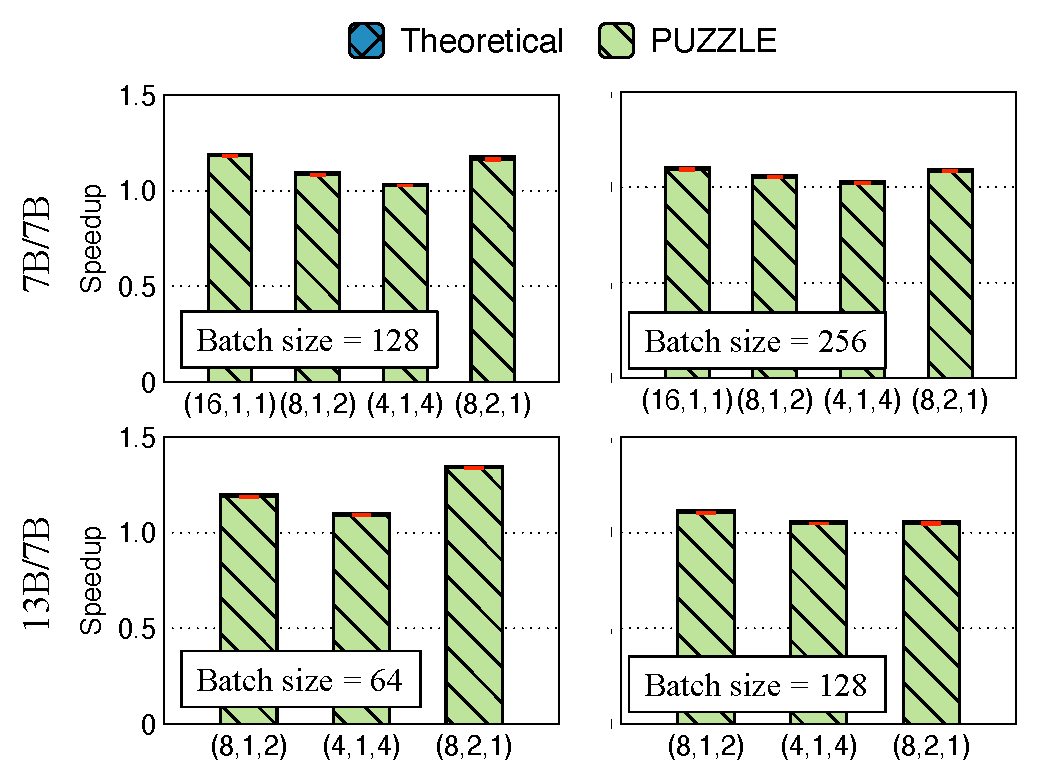
\includegraphics[width=0.65\linewidth]{figures/puzzle/intra-stage-theoreitcal.pdf}
     \caption{阶段内切换的理论加速比与PUZZLE的加速比} 
     \label{fig:intra-stage-theoretical}
\end{figure}

\subsection{阶段间消融实验}  

本研究现在评估 PUZZLE 中涉及阶段间上下文切换的并行执行计划转换所带来的性能提升,评估遵循\Cref{table:end2end-config} 中的配置。
实验以固定的生成最优和训练最优并行执行计划(与 PUZZLE-Base 相同)作为对比基准。\Cref{fig:inter-stage-ablation-study} 展示了各种设置下的端到端加速比。  

与生成最优计划相比,PUZZLE 实现了 1.22倍 的平均加速比;与训练最优计划相比,平均加速比达 1.34倍,开销将在下文的实验展示。
此外,本研究发现生成最优策略始终优于训练最优策略,主要因为生成阶段通常更耗时,因此选择合适的生成计划更为关键。在通信吞吐量更高的 phoenix 配置中,加速比更大,这归因于生成期间张量并行的机会更多。  

这进一步表明,仅基于单一工作负载特性选择并行策略不足以实现最优性能,而最优方法需要综合考虑各种工作负载的特性,并考虑过渡期间的开销,以提升对齐过程的性能。  

\begin{figure}[t]
     \centering
     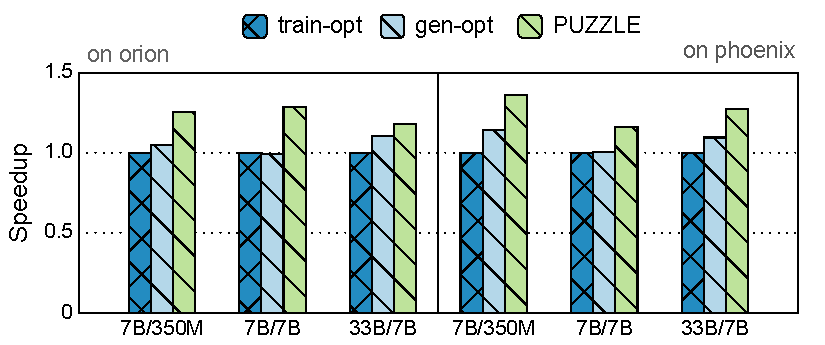
\includegraphics[width=0.65\linewidth]{figures/puzzle/inter-stage-ablation-study.pdf}
     \caption{PUZZLE策略与单阶段最优并行策略的性能比较} 
     \label{fig:inter-stage-ablation-study}
\end{figure}

\subsection{性能分解分析}  

本研究还进行了细粒度性能分解分析,将其与 DeepSpeed-Chat 对比,同时也包含了 PUZZLE-Base 的分析。
研究针对两种集群配置下的 7B/7B 对齐,结果如\Cref{fig:perf-breakdown} 所示,其中分别测量了每个阶段的性能。  

\begin{figure}[t]
     \centering
     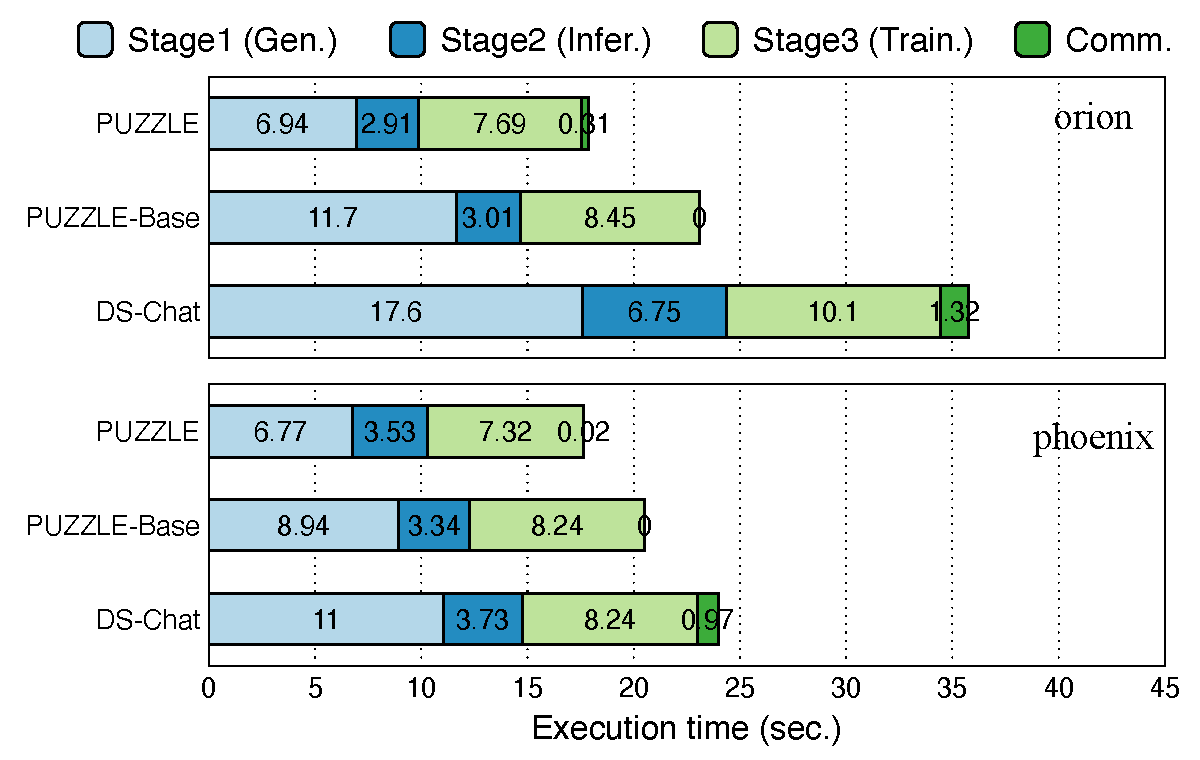
\includegraphics[width=0.7\linewidth]{figures/puzzle/perf-breakdown.pdf}
     \caption{细粒度性能分解分析}
     \label{fig:perf-breakdown}
\end{figure}

实验结果表明,PUZZLE 在各个阶段均优于 DeepSpeed-Chat。
本研究分别讨论这三个阶段性能优化的原因:
在阶段 1,PUZZLE 使用轻量级并行执行计划转换以选择最优策略,相比流水线并行更倾向于张量并行,从而提升性能;
而 DeepSpeed-Chat 仅使用张量并行导致性能较低。
对于阶段 2 和 3,PUZZLE 通过选择合适的放置和执行计划实现显著提升,阶段 2 的增益尤为明显;
阶段 3 的有效性通过时间共享技术进一步提升性能。  

\begin{table}[h]
\caption{阶段间切换开销分析}
\label{table:switch-overhead}
\centering
% \footnotesize
\small
\begin{tabular}{lcccc}
\toprule
\multirow{2}{*}{Config.} & \multicolumn{2}{c}{\textit{orion}} & \multicolumn{2}{c}{\textit{phoenix}} \\ %\cline{2-5}
           & PUZZLE & DS-Chat       & PUZZLE  & DS-Chat       \\ \hline
7B/350M    &  0.31 s     & 1.32 s        & 0.02 s       & 1.03 s        \\
13B/350M   &  0.37 s     & 3.02 s        & 0.20 s       & 2.02 s        \\
33B/7B   &  0.49 s     & 7.54 s        & 0.48 s       & 3.37 s        \\ \bottomrule
\end{tabular}
\end{table}

\Cref{table:switch-overhead} 详细列出了通信开销,对比了 PUZZLE 和 DeepSpeed-Chat 在两个不同集群中的开销。
实验中的阶段间切换主要针对 \texttt{Actor}模型,仅更改 \texttt{Actor} 的参数,其它遵循\Cref{table:end2end-config} 中的配置。  
如表所示,PUZZLE 在两个集群中的开销均低于 DeepSpeed-Chat,且均小于 1 秒。尤其在 \textit{orion} 集群中,33B/7B 配置下,33B 模型参数相对较大且分布在 32 个 GPU 上,DeepSpeed-Chat 的切换开销高达 7.54 秒,而 PUZZLE 以最小开销完成了从 (32,1,1) 到 (16,1,2) 的切换,仅耗时 0.49 秒。
同时,在 \textit{phoenix} 集群中,切换到 (8,1,4) 虽增加了开销,但也显著提升了性能。
这表明 PUZZLE 在各种集群配置下均能有效平衡开销与性能优化。
此外,在 \textit{phoenix} 集群中,由于大部分通信在节点内完成,PUZZLE 有效利用了 NVLink 的通信优势,从而降低了开销。

% \subsection{实验设置}
% 本研究在多个配备不同数量 NVIDIA A100 GPU 的集群上对 PUZZLE 进行评估,集群的 GPU 数量从 8 个到 32 个不等,每个 GPU 具有 80GB 内存。实验中,本研究以 LLaMA-7B、LLaMA-13B 和 LLaMA-30B 等基于 Transformer 架构的大语言模型为对象,使用 PyTorch 作为深度学习框架,并将 PUZZLE 与最先进的基于人类反馈的强化学习训练系统 DeepSpeed-Chat 进行对比。
% 在数据集方面,本研究采用了多个公开的大规模数据集,包括用于生成训练数据的 CommonCrawl 语料库,以及用于构建奖励模型的人工标注数据集。训练过程中,本研究使用近端策略优化(PPO)算法进行大语言模型对齐,并根据模型规模和数据集特点,合理调整超参数,如学习率设置在 \(1e^{-5}\) 到 \(5e^{-5}\) 之间,批次大小根据 GPU 内存和模型复杂度进行动态调整。
% \subsection{性能对比}
% 图 6 展示了 PUZZLE 与 DeepSpeed-Chat 在不同模型规模和 GPU 数量下的端到端训练时间对比。结果表明,PUZZLE 在所有测试场景下均显著优于 DeepSpeed-Chat。当使用 8 个 GPU 对 LLaMA-7B 模型进行对齐训练时,PUZZLE 的训练时间比 DeepSpeed-Chat 缩短了 42\%;随着 GPU 数量增加到 32 个,在对 LLaMA-30B 模型进行训练时,PUZZLE 的加速比最高可达 2.12 倍。平均而言,与 DeepSpeed-Chat 相比,PUZZLE 在不同模型和 GPU 配置下的训练时间平均减少了 58\%,这充分证明了 PUZZLE 在提高大语言模型对齐效率方面的有效性。
% \subsection{开销分析}
% 本研究进一步分析了 PUZZLE 在阶段内和阶段间上下文切换过程中的开销,并与 DeepSpeed-Chat 进行对比。图 7(a)展示了阶段内上下文切换的空闲时间占比情况。可以看到,DeepSpeed-Chat 由于采用传统的顺序执行或简单的并行方案,阶段内存在大量空闲时间,平均空闲时间占比达到 35\%;而 PUZZLE 通过基于亲和性的时间共享切换方案和混合方案,有效减少了空闲时间,平均空闲时间占比仅为 12\%,显著提高了计算资源的利用率。
% 在阶段间上下文切换方面,图 7(b)显示了不同方案切换时的通信成本和参数重组成本。DeepSpeed-Chat 在切换并行执行方案时,由于没有考虑方案之间的相似性,导致通信成本和参数重组成本较高;相比之下,PUZZLE 采用基于相似性的阶段间切换策略,能够选择相似性高的方案进行切换,使得通信成本降低了 60\%,参数重组成本降低了 55\%。这些结果表明,PUZZLE 通过优化阶段内和阶段间的上下文切换,有效降低了整体开销,从而实现了更高的训练效率。
% \subsection{扩展性评估}
% 为了评估 PUZZLE 的扩展性,本研究测试了其在不同规模集群和模型上的性能表现。图 8 展示了随着 GPU 数量增加,PUZZLE 和 DeepSpeed-Chat 的训练吞吐量变化情况。结果显示,PUZZLE 在不同规模的集群上都能保持良好的扩展性,随着 GPU 数量从 8 个增加到 32 个,其训练吞吐量线性增长,增长幅度达到 2.8 倍;而 DeepSpeed-Chat 在 GPU 数量较多时,由于上下文切换开销的增加,扩展性受到限制,吞吐量增长幅度仅为 1.5 倍。这表明 PUZZLE 能够更好地适应大规模集群环境,在处理大规模大语言模型对齐任务时具有显著优势。
% \section{相关工作}
% \subsection{大语言模型训练优化}
% 近年来,众多研究致力于大语言模型的训练优化。一些工作聚焦于改进并行计算策略,例如 Megatron-LM [18] 通过混合并行化方法,结合数据并行、张量并行和流水线并行,有效提升了大语言模型的训练效率;PipeDream [5] 提出了一种新的流水线并行调度算法,减少了 “流水线气泡” 带来的性能损失。还有研究关注计算图优化,如 TensorRT [10] 通过对深度学习模型的计算图进行优化和加速,提高了推理和训练的速度。然而,这些研究主要针对单个模型的训练,对于大语言模型对齐过程中涉及的多个异构模型和频繁上下文切换的场景关注较少。
% \subsection{多模型协同训练}
% 在多模型协同训练领域,已有一些研究探索了不同模型之间的协作和资源分配。例如,一些工作提出了多模型并行训练框架,通过合理分配计算资源和数据,实现多个模型的并发训练 [16, 23]。但这些研究大多假设模型具有相似的结构和工作负载,没有充分考虑大语言模型对齐中模型和工作负载的高度异构性,以及由此带来的频繁上下文切换问题。
% \subsection{上下文切换优化}
% 在计算机系统领域,上下文切换优化一直是一个重要的研究方向。在操作系统中,通过采用快速上下文切换算法和内存管理技术,减少进程或线程切换的开销 [3, 25]。在深度学习领域,也有一些研究尝试优化模型在不同任务或工作负载之间的切换效率 [8, 27]。然而,这些研究与大语言模型对齐中的上下文切换存在本质区别,大语言模型对齐中的上下文切换涉及多个异构模型、复杂的并行执行方案和大量的参数更新与数据传输,需要更针对性的优化策略。

\section{结论}
本研究针对大语言模型对齐过程中异构上下文之间的高效切换这一关键挑战,提出了一个高效的大语言模型对齐系统PUZZLE。
通过深入分析对齐过程的特点,本研究抽象出上下文的概念,并从阶段内和阶段间两个维度进行研究。
在阶段内,本研究提出基于亲和性的时间共享切换方案和混合方案,通过探索上下文之间的亲和性,实现计算重叠,有效减少了阶段内上下文切换的空闲时间和开销;在阶段间,本研究制定了基于相似性的切换策略,通过度量并行执行方案的相似性并搜索最优方案,降低了阶段间上下文切换的通信成本和参数重组成本。
实验结果表明,与最先进的 RLHF 训练系统 DeepSpeed-Chat 相比,PUZZLE 在不同模型规模和 GPU 配置下均实现了显著的性能提升,加速比最高可达 2.12 倍,同时有效降低了上下文切换开销,具有良好的扩展性。
